The list of robot's main hardware components:

\begin{itemize}
  \item Raspberry Pi Model B Board (see Fig. \ref{fig:rpi_board})
  \item Raspberry Pi No-IR Camera
  \item RD02 Robot drive system
  \item Ultrasound Proximity sensor
  \item I2C Breakout Board
\end{itemize}

\begin{figure}[h!]
\centering 

	\begin{subfigure}[h]{0.45\textwidth}
		\centering
			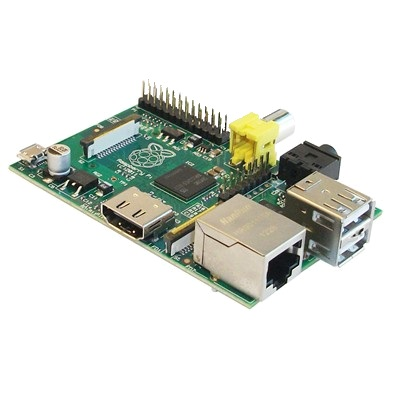
\includegraphics[width=\textwidth]{rpi.png}
			\subcaption{Raspberry Pi Model B board}
			\label{fig:rpi_board}
	\end{subfigure}
	\begin{subfigure}[h]{0.45\textwidth}
		\centering
			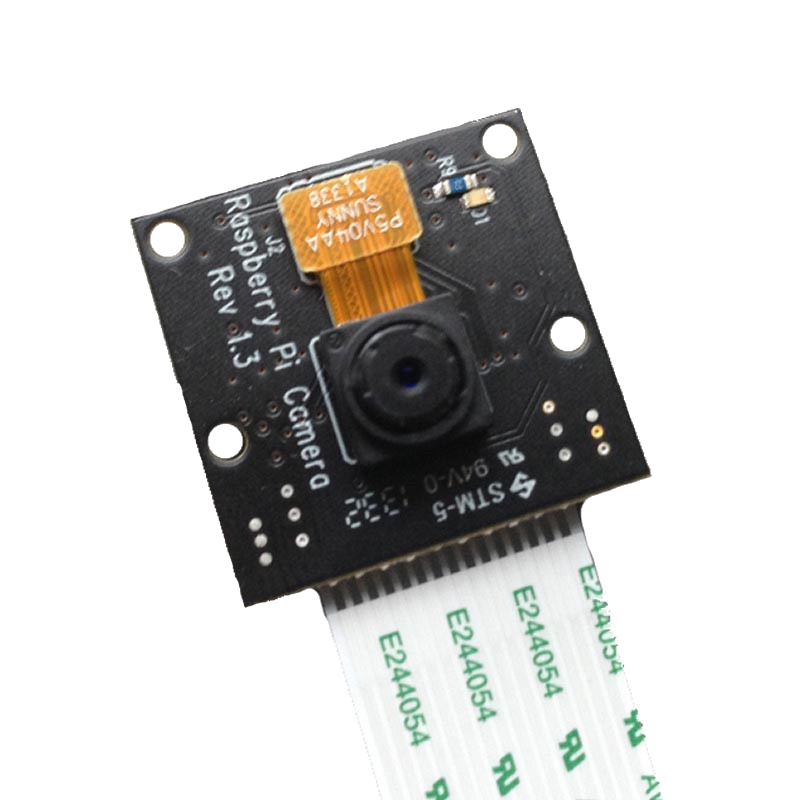
\includegraphics[width=\textwidth]{noir.png}
			\subcaption{Raspberry pi NoIR camera module}
			\label{fig:rpi_noir}
	\end{subfigure}

\caption{Raspberry Pi and NoIR camera}
\label{fig:rpi}
\end{figure}

\subsection*{Mechanical Part} 

The robot drive unit RD02 used in this project consists of MD25 motor control
board, two EMG30 modules (motor, gearbox and a mounting bracket) and two 100mm
wheels (see Fig. \ref{fig:rd02}).

The frame of the robot consists of aluminum profiles and a perforated plate that
serves as a base for mounting electronic components. Two driving wheels
are mounted on a EMG30 gearbox shaft that connected to the frame via the
provided bracket. A metal ball wheel is located in front of the robot and
provides remaining support.

EMG30 is a module that incorporates motor, gearbox and encoder with Hall sensor.
It is suited for medium robotics applications. The gearbox provides increased
torque allowing robust movement in different environments while the Hall sensor
obtains information about the rotation of the shaft.

\begin{figure}[h!]
\centering 

	\begin{subfigure}[h]{0.45\textwidth}
		\centering
			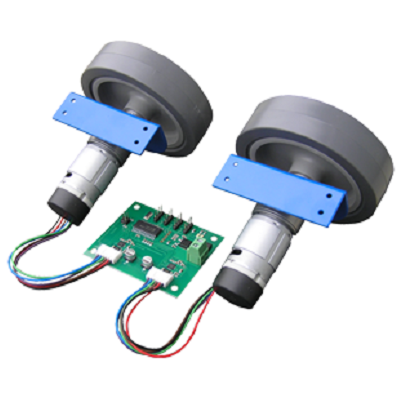
\includegraphics[width=\textwidth]{rd02.png}
			\subcaption{RD02 Robot Drive System}
			\label{fig:rd02}
	\end{subfigure}
	\begin{subfigure}[h]{0.45\textwidth}
		\centering 
			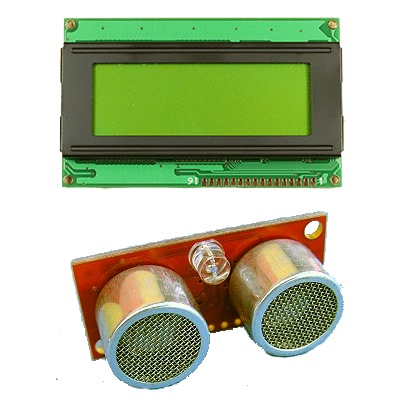
\includegraphics[width=\textwidth]{lcd.png}
			\subcaption{20x4 LCD Module and ultrasonic range sensor}
			\label{fig:lcd_us}
	\end{subfigure}

\caption{RD02 Robot Drive System}
\label{fig:modules}
\end{figure}

\subsection*{Electronics}
 
The main electronic component of the robot is the Raspberry Pi Model
B single-board computer. Its technical specifications are listed in the Table
\ref{tab:rpi_specs}.

\begin{table}[h!]
	\setlength\extrarowheight{2pt}
    \begin{tabularx}{\textwidth}{XX}
    
    ~                 & ~                                                           \\
    System on a chip  & Broadcom BCM2835                                            \\
    CPU               & 700 MHz ARM11                                               \\
    GPU               & Broadcom VideoCore IV @ 250 MHz                             \\
    RAM               & 512 Mb shared with GPU                                      \\
    Memory            & SD Card Slot                                                \\
    Ports             & 2x USB, LAN, 3.5mm phone jack, HDMI,  GPIO (UART, I2C, SPI) \\
    Power Consumption & 700 mA (3.5 W)                                              \\
    
    \end{tabularx}
    \caption{Raspberry Pi Model B Specifications}
    \label{tab:rpi_specs}
\end{table}

The board is running an adapted version of the Debian Linux distribution. The
development can either be performed on the board itself after connecting the
necessary peripherals, or via remote connection such as SSH.

The board is powered using 11.1V Turnigy LiPo Battery via power adapter that
splits the voltage into 12V (motors) and 5V lines. According to the external
power supply measurements, the average total consumption during movement is
approximately 8W.

The Raspberry Pi peripherals include a WiFi adapter, GPIO breakout board for
simplifying the connection of other modules, and a Raspberry Pi camera (see
Fig. \ref{fig:rpi_noir}).
RPi camera is a board-specific 5Mp camera module connected via 15-pin MIPI (Mobile Industry
Processor Interface) connector. It is capable of capturing 1080p video and
perform basic hardware video processing. Two different types of cameras were
tested - standard camera and near-IR ``NoIR'' camera with the infrared filter
removed.
The performance comparison of different cameras is shown in the Table
\ref{tab:cam_perf}.  In order to increase the reliability and robustness of 
NoIR camera, a couple of IR LEDs were installed to provide additional illumination.

After a series of experiments, the signs were made of a highly-reflective duct
tape that showed high reflectance under poor lighting
conditions. The usage of the NoIR camera accompanied with a couple of IR LEDs
showed high segmentation performance with minimum lighting provided.

MD25 is a dual H-Bridge I2C / Serial motor driver suited for the control of
EMG30 modules.
It provides additional capabilities in the motor manipulation, such as variable
acceleration, motor current information and independent control of two motors
with encoder feedback. It is also equipped with a 5V regulator, however it is
impossible to power the Raspberry Pi as the continuous supply rate is 300 mA,
while the average consumption of Raspberry Pi is 700 mA.

Due to the reason explained before, Raspberry Pi is powered using Taco Power TSR
1-2450 DC-DC voltage step-down modules that provide 5V 1A output.

% Fix table here
\begin{table}[h!]
	\setlength\extrarowheight{2pt}
	\setlength\arraycolsep{5pt}
    \begin{tabularx}{\textwidth}{XXXX}
    Resolution / Camera Setup & Raspberry Pi  (CPU) + Raspberry Pi Camera &
    Raspberry Pi (CPU) + Logitech C270 & Odroid-U3 (CPU) + Logitech C270 \\
    160x120            & 18           & 9          & 30         \\
    320x240            & 6            & 4.8        & 20         \\
    640x480            & 2.5          & 2.3        & 11         \\
    1280x720           & 0.6          & 0.8        & 4          \\
    \end{tabularx}
    \caption{Camera Performance comparison}
    \label{tab:cam_perf}
\end{table}

As can be seen from the Table \ref{tab:cam_perf}, the main advantage of using
RPi camera is its performance - it outperforms generic Webcam grace to hardware
optimization and, in particular, absence of resizing routine in the code.
However, the disadvantage lies in the specificity of the camera, that can only
be used on the RPi board, while the USB Webcam can be used everywhere, so in
order to port the solution to another platform, the camera change as well as
 code modification are required.

The robot is also equipped with an ultrasound proximity sensor used for obstacle
detection. It is a basic proximity sensor with a focus of 15 degrees and an
accuracy about 2mm. An I2C LCD Screen module provides an interface for visual feedback.
These components are shown on the Fig. \ref{fig:lcd_us0}.